\documentclass[a4paper]{article}
\usepackage{cite}
\usepackage{amsmath}
\usepackage{graphicx}
\usepackage{listings}
\usepackage[usenames,dvipsnames]{color}
\usepackage{dsfont}

\definecolor{gray}{cmyk}{0,0,0,0.50}
\definecolor{Brown}{cmyk}{0,0.81,1,0.60}
\definecolor{OliveGreen}{cmyk}{0.64,0,0.95,0.40}
\definecolor{CadetBlue}{cmyk}{0.62,0.57,0.23,0}
\definecolor{lightlightgray}{gray}{0.9}


\author{Dmitry Serdyuk}
\title{Assignment 3}
\date{}
\renewcommand{\vec}[1]{\mathbf{#1}}

\begin{document}
\lstset{
language=Python,                             % Code langugage
basicstyle=\ttfamily,                   % Code font, Examples: \footnotesize, \ttfamily
keywordstyle=\color{OliveGreen},        % Keywords font ('*' = uppercase)
commentstyle=\color{gray},              % Comments font
numbers=left,                           % Line nums position
numberstyle=\tiny,                      % Line-numbers fonts
stepnumber=1,                           % Step between two line-numbers
numbersep=5pt,                          % How far are line-numbers from code
backgroundcolor=\color{lightlightgray}, % Choose background color
frame=none,                             % A frame around the code
tabsize=2,                              % Default tab size
captionpos=b,                           % Caption-position = bottom
breaklines=true,                        % Automatic line breaking?
breakatwhitespace=false,                % Automatic breaks only at whitespace?
showspaces=false,                       % Dont make spaces visible
showtabs=false,                         % Dont make tabls visible
}

\section{Induced graphs}

Let's proove, that if there is a path described in the task, then there is a fill edge $X$ -- $Y$.
If we run the variable elimination algorithm on the graph $H$ and pause it after the algorithm would
eliminate all $Z_i$ but wouldn't eliminate $X$ and $Y$. It is possible because all $Z_i$ go before
$X$ and $Y$. At this point we should have a $\tau$ which depends on $X$ and $Y$ which "contains" all
the factors $\Phi(X, Z_1, \ldots)$, $\Phi(Z_i, Z_{i+1}, \ldots)$, $\Phi(Z_k, Y, \ldots)$. In other
words, we should have a fill edge $X$ -- $Y$ by definition of a fill edge.


Otherwise, if we have that $X$ -- $Y$ is a fill edge, we consider a $\tau$ from the definition of
a fill edge. Let's suppose, that $Z_{i_1}$ is a variable which was eliminated when $\tau$ was created,
this variable was eliminated before $X$ and $Y$.
Consider two pairs of variables ($X$, $Z_{i_1}$) and ($Z_{i_1}$, $Y$). There are only two possibilities for
each pair ($A$, $B$): either $A$ -- $B$ is a fill edge or $A$ -- $B$ is an edge in graph $H$, otherwise
$X$ -- $Y$ is not a fill edge. We can apply the same argument for each pair recurcevely. Then we reorder 
$Z_{i_k}$ from $X$ to $Y$ and this is a path we would like to find: every $Z_{i_k} \prec X, Y$.

\section{HMM}

\subsection{(a) Update equations}

\begin{align*}
\delta_{y_t \rightarrow x_t}(x_t) &=& \sum_{y_t} \mathrm{Pr}\left[ y_t | x_t \right] 
\mathds{1} \left[y_t = \hat{y}_t\right] \\
\delta_{x_{t - 1} \rightarrow x_t}(x_t) &=& \sum_{x_{t - 1}} \mathrm{Pr}\left[ x_t | x_{t - 1} \right] 
\delta_{y_{t-1} \rightarrow x_{t - 1}}(x_{t-1}) \delta_{x_{t - 2} \rightarrow x_{t - 1}}(x_{t - 1}) \\
\delta_{x_{t + 1} \rightarrow x_{t}}(x_t) &=& \sum_{x_{t + 1}} \mathrm{Pr}\left[ x_{t + 1} | x_t \right]
\delta_{y_{t + 1} \rightarrow x_{t + 1}}(x_{t + 1}) \delta_{x_{t + 2} \rightarrow x_{t + 1}}(x_{t + 1}) \\
\delta_{x_t \rightarrow y_t}(y_t) &=& \sum_{x_t} \mathrm{Pr} \left[ y_t | x_t \right] 
\delta_{x_{t + 1} \rightarrow x_t}(x_t)
\end{align*}


\subsection{(b) Implementation}

Here is implementation:
\begin{lstlisting}[language=Python]
# x = 'bad' <=> 0, x = 'good' <=> 1
# y = -1 <=> 0, y = 1 <=> 1
message_y_x = np.zeros((n, 2))
message_x_fort = np.zeros((n, 2))
message_x_back = np.zeros((n, 2))
message_x_y = np.zeros((n, 2))

# Probability x_{t + 1} given x_t
prob_x_x = np.array([[0.8, 0.2],
                     [0.2, 0.8]])
# Probability x_t given y_t
prob_x_y = np.array([[q_value, (1 - q_value)],
                     [(1 - q_value), q_value]])
# Probability x_1
prob_x1 = np.array([1 - prob_x1, prob_x1])

# Backward pass
for i in reversed(xrange(0, n)):
    if data[i] == -1:
        message_y_x[i, 0] = q_value
        message_y_x[i, 1] = 1. - q_value
    else:
        message_y_x[i, 0] = 1. - q_value
        message_y_x[i, 1] = q_value

    if i == n - 1:
        message_x_back[n - 1, :] = (message_y_x[n - 1, 0] * prob_x_x[0, :] +
                                    message_y_x[n - 1, 1] * prob_x_x[1, :])
        continue

    message_x_back[i, :] = (message_y_x[i, 0] * message_x_back[i + 1, 0] * prob_x_x[0, :] +
                            message_y_x[i, 1] * message_x_back[i + 1, 1] * prob_x_x[1, :])

# Forward pass
for i in xrange(0, n):
    if i == 0:
        message_x_y[0, :] = (prob_x_y[1, :] * message_x_back[1, 1] * prob_x1[1] +
                             prob_x_y[0, :] * message_x_back[1, 0] * prob_x1[0])
        message_x_fort[0, :] = (prob_x_x[:, 1] * message_y_x[0, 1] * prob_x1[1] +
                                prob_x_x[:, 0] * message_y_x[0, 0] * prob_x1[0])
        continue
    if i == n - 1:
        message_x_y[n - 1, :] = (prob_x_y[1, :] * message_x_fort[n - 2, 1] +
                                 prob_x_y[0, :] * message_x_fort[n - 2, 0])
        message_x_fort[n - 1, :] = (prob_x_x[:, 1] * message_y_x[n - 1, 1] * message_x_fort[n - 2, 1] +
                                    prob_x_x[:, 0] * message_y_x[n - 1, 0] * message_x_fort[n - 2, 0])
        continue
    message_x_y[i, :] = (prob_x_y[1, :] * message_x_back[i + 1, 1] * message_x_fort[i - 1, 1] +
                         prob_x_y[0, :] * message_x_back[i + 1, 0] * message_x_fort[i - 1, 0])
    message_x_fort[i, :] = (prob_x_x[:, 1] * message_y_x[i, 1] * message_x_fort[i - 1, 1] +
                            prob_x_x[:, 0] * message_y_x[i, 0] * message_x_fort[i - 1, 0])

# Normalisation
message_y_x /= np.sum(message_y_x, axis=1).reshape((-1, 1))
message_x_fort /= np.sum(message_x_fort, axis=1).reshape((-1, 1))
message_x_back /= np.sum(message_x_back, axis=1).reshape((-1, 1))
message_x_y /= np.sum(message_x_y, axis=1).reshape((-1, 1))
\end{lstlisting}

\begin{figure}
    \begin{center}
        \includegraphics[width=6cm]{prob_07.eps}
        \caption{Probablities of having $x = "good"$ with $q=0.7$}
        \label{fig:hmm07}
    \end{center}
\end{figure}

\begin{figure}
    \begin{center}
        \includegraphics[width=6cm]{prob_09.eps}
        \caption{Probablities of having $x = "good"$ with $q=0.9$}
        \label{fig:hmm09}
    \end{center}
\end{figure}

\subsection{(c) Results $q=0.7$}
The results are shown on Fig.~\ref{fig:hmm07}. The probability to have a good economic state 
during the week $39$ is $0.7849$.

\subsection{(d) Results $q=0.9$}
The results are shown on Fig.~\ref{fig:hmm09}. The probability to have a good economic state
during the week $39$ is $0.9551$. We can see, that the data have more impact on the results
with $q=0.9$. 

\section{}
\section{Gibbs sampling}
\subsection{(a) Conditional probability}

\begin{align*}
& \mathrm{Pr}\left[x_{i, j} = 1 | all\ others\right] 
= \mathrm{Pr}\left[x_{i, j} = 1| x_{i - 1, j}, x_{i, j - 1}, x_{i + 1, j}, x_{i, j + 1}\right] \\
&= \exp(\theta x_{i, j} x_{i - 1, j} + \theta x_{i, j} x_{i, j - 1} + \theta x_{i, j} x_{i + 1, j} + \theta x_{i, j} x_{i, j + 1}),
\end{align*}
where $x_{k, l} = 0$ if $k$ or $l$ is an invalid index.


\subsection{(b) Gibbs sampling}
The code for Gibbs sampling in Ising model:
\begin{lstlisting}[language=Python]
rng = np.random.RandomState(123)
vars = (rng.binomial(1, 0.5, size=(size, size)) * 2) - 1
ans = []
for it in xrange(num_iter):
    for i in xrange(size):
        for j in xrange(size):
            sum = 0
            if i != 0:
                sum += theta * vars[i - 1, j]
            if i != size - 1:
                sum += theta * vars[i + 1, j]
            if j != 0:
                sum += theta * vars[i, j - 1]
            if j != size - 1:
                sum += theta * vars[i, j + 1]
            prob_neg = np.exp(-sum)
            prob_pos = np.exp(sum)
            sample = rng.binomial(1, prob_pos / (prob_neg + prob_pos))
            vars[i, j] = (sample * 2) - 1
\end{lstlisting}
The result are shown in the Fig.~\ref{fig:gibbs}.

\subsection{(c) Inference in tree-structured graph}

It is always possible to consider a tree-like undirected model as a directed model with the 
same geometry and conditional probabilities given by 
\begin{equation}
\mathrm{Pr}\left[ x | \mathrm{Pa}(x)\right] = \frac{1}{Z} \Phi(x) \Phi(x, Pa(x)),
\label{eq:fact}
\end{equation}
where $\mathrm{Pa}(x)$ is the only parent of $x$, $\Phi(x)$ and $\Phi(x, Pa(x))$ are factors 
associated with $x$ and the parent of $x$. $Z = \sum \Phi(x) \Phi(x, Pa(x))$ is the normalization constant.

Since we can describe the model in terms of Bayesian net, we can sample from it using 
ancestral sampling. More presisely, we can sample from the root $x_1$ according to probability
$\mathrm{Pr}[x_1]$, then sample all the children of $x_1$ using conditional probabilities defined 
in Eq.~\ref{eq:fact}. Then we recursively repeat the procedure to the next layer of children.

\subsection{(d) Block Gibbs sampling}

We can use ancestor sampling to sample from a part of the graph. Then we fix this part and perform 
ancestor sampling from the other part. Then we repeat the procedure.

\subsection{(e) Implementation of block Gibbs sampling}

Here is python code for sampling:
\begin{lstlisting}[language=Python]
ng = random.RandomState(1)
vars = rng.binomial(1, 0.5, (size, size)) * 2. - 1.
probs = np.zeros((size, size))

def do_ancestral_sampling(vars, iterator, theta):
    cur_iter = iterator()
    next_iter = iterator()
    next_iter.next()
    for (i, j), nind in izip_longest(cur_iter, next_iter):
        neigh = neighbours(i, j, size)
        if nind is not None:
            neigh = neigh.difference(nind)
        energy = 0.0
        for ii, jj in neigh:
            energy += vars[ii, jj]
        prob_pos = np.exp(theta * energy)
        prob_neg = np.exp(-theta * energy)
        prob_pos, prob_neg = (prob_pos / (prob_neg + prob_pos),
                              prob_neg / (prob_neg + prob_pos))
        probs[i, j] = prob_pos
        vars[i, j] = rng.binomial(1, prob_pos) * 2. - 1.
        
        
for i in xrange(num_iter):
    do_ancestral_sampling(vars, tree_iter(0, size), theta)
    do_ancestral_sampling(vars, tree_iter(1, size), theta)
\end{lstlisting}

Result are shown on Fig.~\ref{fig:block_gibbs}.

Both samplers output correlated samples from my point of view but it seems to me, that 
block Gibbs samples seems to mix better.

\begin{figure}
    \begin{center}
        \includegraphics[width=15cm,height=6cm]{samples.eps}
        \caption{Gibbs sampling results. Samples were drawn every $100$ iterations.}
        \label{fig:gibbs}
    \end{center}
\end{figure}

\begin{figure}
    \begin{center}
        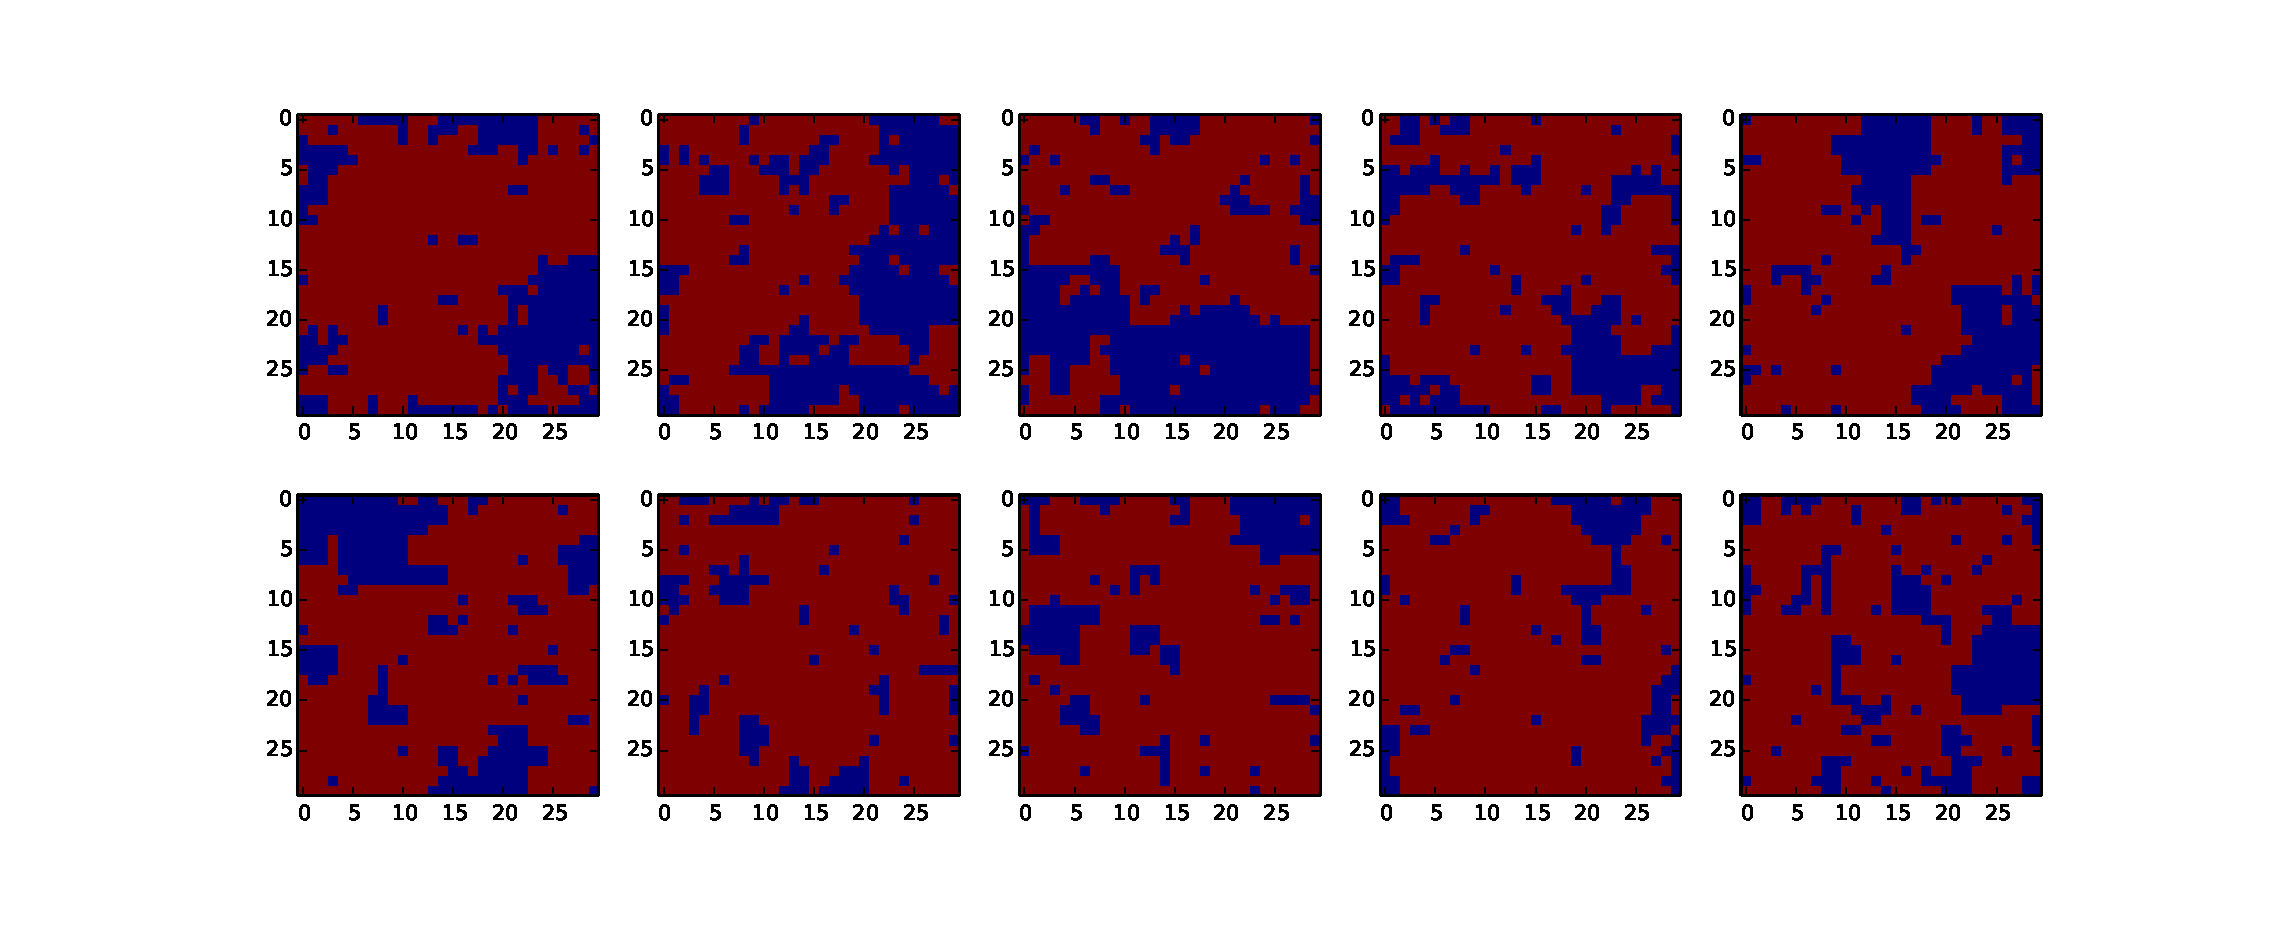
\includegraphics[width=15cm,height=6cm]{sample_block.eps}
        \caption{Block Gibbs sampling results using acestral sampling for sampling from each block. 
        Samples were drawn every $100$ iterations.}
        \label{fig:block_gibbs}
    \end{center}
\end{figure}
\end{document}
